% !TeX spellcheck = en_GB
%****************************************************
%	CHAPTER  - Implementation
%****************************************************
\chapter{Implementation}
\label{ch:implementation}
This chapter provides a detailed description of each module used in the multi-robot multi-session system to generate a global map on each team's mobile robot. 

\section{Overview}

In this work, a multi-robot, multi-session map merging algorithm capable of merging maps of different resolutions, is presented. Each robot in the system can generate a local and global map, hence it is a distributed system. Hector SLAM is used to generate the local maps, which are inputs to the map merging algorithm that produces a global map. A map merging algorithm is presented. The implementation of the algorithm is then presented for real-time capability. The map merging algorithm has input maps from other robots in the network and previously mapped session, enabling the robot to deal with multiple session mapping. 

\section{Map merging algorithm}
\label{sec:map_merging_algorithm}

This section describes the map merging algorithm used in this thesis, which is based on image registration. The image registration is transforming different images into the same coordinate system, using the following steps feature detection, matching, alignment and merging. In this work, occupancy grid maps are represented as images where a pixel defines whether an area is occupied, unoccupied or unknown. These images can be taken at multiple resolutions, viewpoints, and using different sensors; therefore, the spatial relationships or the maps include rotation, translation and scaling. As described in the previous chapter Scale-invariant feature transform (SIFT) will be used as a feature detector as it deals well with the spatial relationship described above. 

OpenCV was started at Intel in 1999 by Gary Bradsky, however, the first release in 2000 when it was used on Stanley (the vehicle that won the DARPA Grand Challenge that year). OpenCV is supported in C++, Python and Java; hence it can be used across various systems. The Python API of OpenCV (OpenCV-Python) is used to implement the solution; the API includes a wide range of tools such as feature detection, object detection, machine learning and video analysis. The image registration module used in this work is based on Scale-invariant feature transform (SIFT), results presented in Chapter \ref{sec:map-merging} show that it is superior for this scenario. The scale and rotation invariant nature of SIFT, it can be used in multi-resolution scenarios.

Feature detection, matching features, and alignment are included and merging the maps to form a global map.

\subsection{Transformation}
Assume there are two maps $map_1$ and $map_2$, where $map_1$ is the local map of $robot_1$ and consequently $map_2$ is the local map of $robot_2$. This section describes the process of transforming $map_2$ into $map_1$'s frame of reference. Algorithm \ref{alg:1} describes this process.

\begin{algorithm}
\SetAlgoLined
\SetNoFillComment
\DontPrintSemicolon

\tcc{This function transforms $map_2$ into $map_1$'s frame. The function requires two 2D occupancy grid maps of size n by m and RANSAC parameters(confidence, and reproj\_threshold)}


\SetKwProg{Fn}{Function}{}{end}

\Fn{Transform($map_1, map_2, confidence, reproj\_threshold$) : $transformed\_map_2, scale$}{

\tcc{extract feature key-points and corresponding descriptors}
$kp_1$, $des_1$ = detect\_keypoint\_descriptors($map_1$) \;

$kp_2$, $des_2$ = detect\_keypoint\_descriptors($map_2$) \;

\tcc{extract feature matches between two maps}
good\_matches = match\_features($des_1$, $des_2$) \;

\tcc{get feature locations of good matches}
$feature\_locations_1$ = [0, good\_matches.length][0, 2] : 2D array of float \;
$feature\_locations_2$ = [0, good\_matches.length][0, 2] : 2D array of float \;
        
\For{i, match in enumerate(good\_matches)} 
{ 
    $feature\_locations_1$[i, :] = $kp_1$[match.$des_1$\_index].pt \;
    $feature\_locations_2$[i, :] = $kp_2$[match.$des_2$\_index].pt \;
}
\EndFor

\tcc{compute match ratio}
$match\_ratio = good\_match.length/min(kp_1.length, kp_2.length)$ \;
\tcc{compute maximum iterations needed to estimate affine transformation matrix using RANSAC}
$max\_iter = \log(1-confidence)/\log(1-match\_ratio^2)$ \;

\tcc{estimate affine transformation matrix}
affine\_transformation\_matrix = estimate\_affine\_transformation($feature\_locations_1$, $feature\_locations_2$,  $max\_iter$, $confidence$, $reproj\_threshold$) \;

\tcc{transform map using affine transformation matrix}
$transformed\_map_2$ = affine\_transform($map_2$, affine\_transformation\_matrix) \;

\tcc{get scale and angle of rotation from the transformation matrix}
$ss$ = affine\_transformation\_matrix[0, 1] \;
$sc$ = affine\_transformation\_matrix[0, 0] \;
$scale = \sqrt{ss * ss + sc * sc}$\;
$angle\_of\_rotation = \arctan{\frac{ss}{sc}} * 180 / \pi$ \;


\Return $transformed\_map_2$, $scale$ \;
}
\caption{Transform map into main maps frame of reference}
\label{alg:1}
\end{algorithm}

Feature detection is the initial step described in lines 2-3 in algorithm \ref{alg:1}, where a pair of key-points and descriptors are returned (see Chapter \ref{sec:map-merging} for more information). The features are then matched using a Brute-Force Matcher (line 4). The Brute-Force Matcher takes descriptors from each image and matches them using a distance calculation to determine the closest features. In this case the Euclidean distance described by Equation \ref{eq:euclidean_distance} \cite{Lowe2004}. These matches are referred to as $good\_matches$. The $good\_matches$ are then used to get the locations of the features that were $good\_matches$ in lines 5-10. Next, the affine transformation matrix described by Equation \ref{eq:transformation} is computed using RANSAC. In Section\ref{subsec:map_alignment}, parameters $ransacReprojThreshold$ and $maxIters$ were introduced and here we define their values. 

\textbf{$maxIters$} is the maximum number of iterations and is described by the following equation :

\begin{equation}
    1-confidence = (1 - match\_ratio^{n})^{maxIters}
\end{equation}

where, $\{confidence | confidence \in \mathbb{R}, 0 < confidence < 1 \}$, $match\_ratio$ is the ratio of possible matches to good matches described by Equation \ref{eg:nmatch_ratio}, $n$ is the minimum number of features needed for a match \cite{Fischler1981}. By taking the $\log$ of both side get the following equation:

\begin{equation}
    maxIters = \frac{\log(1-confidence)}{ \log(1 - match\_ratio^{n})}.
\end{equation}

Then we choose a $confidence$ of $0.99$ which ensures minimal error, and minimum number of features $n$ of 2, to get:

\begin{equation}
    maxIters = \frac{\log(0.01)}{ \log(1 - match\_ratio^{2})}
\end{equation}


The maximum iterations can then be described by the following Figure \ref{fig:itervsmatch}. Where the smaller the match ratio, the more iterations are required to estimate the best model fit.
\begin{figure}[!h]
\centering
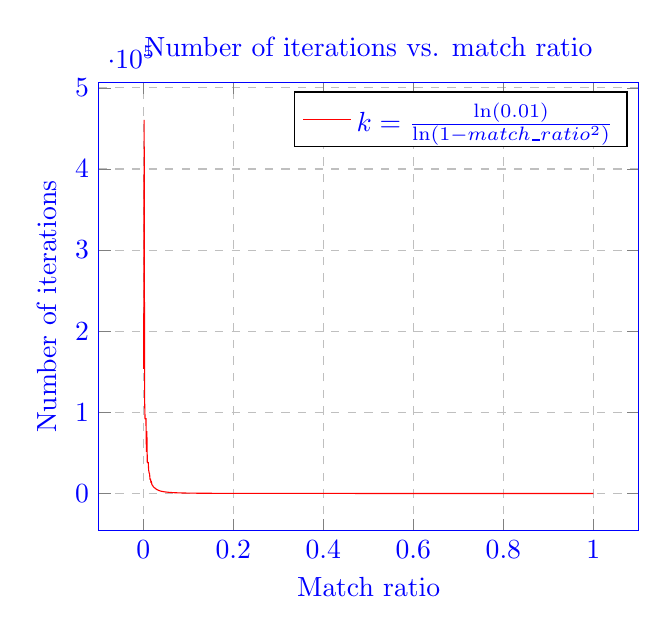
\begin{tikzpicture}

\begin{axis}[
    title={Number of iterations vs. match ratio},
    xlabel={Match ratio},
    ylabel={Number of iterations},
    domain=0:1, 
    samples=1000, 
    color=blue,
    ymajorgrids=true,
    xmajorgrids=true,
    grid style=dashed
]
\addplot[color=red]{-4.60517/(ln(1 - x) + ln(1 + x))};
\legend{$k = \frac{\ln(0.01)}{\ln(1 - match\_ratio^2)}$}
\end{axis}

\end{tikzpicture}
\caption{This figure illustrates the relationship between the number of iterations and the match ratio. The lower the match ratio, the higher the number of iterations. Therefore, lower match ratio matches are computationally costly compared to higher match ratio matches.}
\label{fig:itervsmatch}
\end{figure}

RANSAC uses $ransacReprojThreshold$ in order to determine if a data sample agrees with a model or not. The samples under this threshold will then form that consensus for that model and the data set's inliers if the correct model is found. Hence, it should be chosen according to the model needs. To determine the threshold for this thesis's work, maps in Figure \ref{fig:maps} are paired into groups of two giving a combination of 10. These where then run on line 1 - 14 of algorithm \ref{alg:1}. These maps were then merged and then recorded if the merge was successful if they failed. Table \ref{table:ransacReprojThreshold} shows that $ransacReprojThreshold$ values of 8,9 and 10 show a $100\%$ success rate this work we will use a $ransacReprojThreshold$ value of 9. 


\begin{table}[h]
\small
\setlength\tabcolsep{0.2pt}
\begin{longtable}{|p{2.1cm}|p{1.2cm} p{1.2cm} p{1.2cm} p{1.2cm} p{1.2cm} p{1.2cm} p{1.2cm} p{1.2cm} p{1.2cm} p{1.2cm}|p{2.2cm}|}%{|c|cccccccccc|c|}
\caption[Determining $ransacReprojThreshold$]{Results from running merging on threshold between 1 and 10 to determine the optimal $ransacReprojThreshold$. Where P represents a successful transformation and F a failed transformation.} 
\hline
\multirow{2}{*}{\textbf{Threshold}} & \multicolumn{10}{c|}{\textbf{Combination Num}}                                                    & \multirow{2}{*}{\textbf{P Rate (\%)}} \\ \cline{2-11}
            & 1       & 2       & 3       & 4       & 5       & 6       & 7       & 8       & 9       & 10  &    \\ 
\hline
\endfirsthead
\endhead
\hline
\endfoot
\endlastfoot

1                                   & F & F & P & P & F & P & F & P & P & F & 50                        \\
2                                   & F & F & P & P & F & P & F & P & P & P & 60                        \\
3                                   & P & P & P & P & P & P & F & P & P & P & 90                        \\
4                                   & P & P & P & P & P & P & P & P & F & P & 90                         \\
5                                   & P & P & P & P & P & P & P & P & F & P & 90                         \\
6                                   & P & P & P & P & P & P & P & P & F & P & 90                        \\
7                                   & P & P & P & P & P & P & P & P & F & P & 90                         \\
8                                   & P & P & P & P & P & P & P & P & P & P & 100                       \\
9                                   & P & P & P & P & P & P & P & P & P & P & 100                       \\
10                                  & P & P & P & P & P & P & P & P & P & P & 100                       \\ 
\hline
\label{table:ransacReprojThreshold}
\end{longtable}
\end{table}
Finally, from the affine transformation matrix, the scaling factor and angle of rotation are calculated to be used in further processes. The transformation matrix is of the form:

\begin{align}
M &=
\begin{bmatrix}
cos(\theta)\dot s &  -sin(\theta)\dot s & t_x\\
sin(\theta)\dot s &  cos(\theta)\dot s & t_y 
\end{bmatrix}
\label{eq:rotation-mat}
\end{align}
where, \(\theta\) is the rotation angle, \(s\) the scaling factor and $t_x$,$t_y$ are translations in \textit{x}, \textit{y} axes respectively.

The scaling factor ($s$) and rotation angle ($\theta$)) can be computed using:

\begin{equation}
\begin{split} 
s &=  \sqrt[2]{ M_{1,2}*M_{1,2} + M_{1,1}*M_{1,1} }  \\ 
\theta &= \arctan{(\frac{M_{1,2}}{M_{1,1}})} \times \frac{180}{\pi}
\label{eq:rotat_scale}
\end{split}
\end{equation}.


\subsection{Multiple map transformation}

The \textbf{Transformation} function (algorithm \ref{alg:2})is then used to compute and transform more than one map into the local map's frame of reference. The \textbf{Main} function (algorithm \ref{alg:2}) receives multiple maps and their corresponding resolutions, and then they are merged to form a global map.

\begin{algorithm}[H]
\SetAlgoLined
\SetNoFillComment
\DontPrintSemicolon

\tcc{This is the primary function which receivers all the maps and corresponding scales, then transforms them relative to map[0] and returns the $global\_map$}


\SetKwProg{Fn}{Function}{}{end}

\Fn{Main($maps\_list, map\_resolutions\_list$) : $global\_map$}{
\tcc{initialise variables}
$confidence$ = $0.99$ \;
$reproj\_threshold$ = $9$ \;
$successfully\_transformed\_maps$ = $[]$ \;

\tcc{Loop through maps and transform them relative to $maps\_list[0]$}
\For{$\ i\  in\  range(1, len(maps\_list$))} 
{ 
\tcc{transform map based on the reference $maps\_list[0]$}
$transformed\_map, scale= Transform(map_1, map_2, confidence, reproj\_threshold)$ \;

\tcc{check success of transformation based on resolution}
\If {$(map\_resolutions\_list[0] \times (1-confidence)) > abs(map\_resolutions\_list[0] - (map\_resolutions\_list[i]/scale))$}
{
$successfully\_transformed\_maps.append(transformed\_map)$ \;
}

}

\EndFor

$global\_map = maps\_list[0]$ \;

\tcc{merge only successfully transformed maps}
\For{map in successfully\_transformed\_maps}
{
$global\_map = merge(global\_map, map)$\;
}

\Return $global\_map$\;
}
\caption{Main Function}
\label{alg:2}
\end{algorithm}

Given that not all transformations will be successful, the success is determined by comparing the expected scaling factor and the computed scaling factor. The expected scaling factor is determined by the local map's resolution divided by the resolution of maps from the other robot. This expected scaling factor needs to be within $1 - confidence$, which is the expected RANSAC estimation error. The successful maps are then merged using the following rule in Table \ref{tab:merge-rule}, which allows for a suitable global map to be obtained. If there are one or more successful alignments the map is then returned with it is corresponding resolution.

\begin{table}[H]
\centering
\caption{Rules of Map Merging between two partial maps.}
\begin{tabular}{l|l|c|c|c|c}
\multicolumn{2}{c}{}&\multicolumn{2}{c}{Partial Map 2}\\
\cline{3-5}
\multicolumn{2}{c|}{}&\textbf{Unknown}&\textbf{Free}&\textbf{Occupied}\\
\cline{2-5}
\multirow{2}{*}{Partial Map 1}& \textbf{Unknown} & Unknown & Free & Occupied\\
\cline{2-5}
& \textbf{Free} & Free & Free & Occupied\\
\cline{2-5}
& \textbf{Occupied} & Occupied & Occupied & Occupied\\
\cline{2-5}
\end{tabular}
    
    \label{tab:merge-rule}
\end{table}


\section{ROS implementation}

The algorithm \ref{alg:2} described above is then implemented on the Robot Operating System (ROS) to perform the map merging algorithm in real-time. Figure \ref{fig:systemoverview} describes the system overview of a robot. The robot will receive maps from other robots, maps from previous sessions, and a local map that it produces onboard, and merge them to produce a global map. Each robot must scan the network for possible partial local maps from other robots, to retrieve the maps.

\begin{figure}[H]
    \centering
    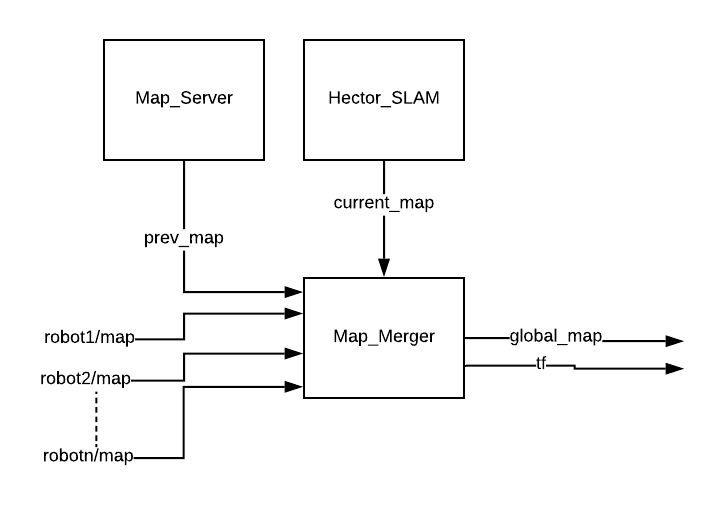
\includegraphics[width=1\textwidth]{figs/ROS_Block_Diagram_2.png}
    \caption{System overview of the solution. The map merging algorithm's inputs included the current partial map ($current\_map$), previous partial map ($prev\_map$), and partial maps of other robots in the environment ($robot1/map, $). The resultant map includes the global map ($global_map&)$ and transformations ($tf$).}
    \label{fig:systemoverview}
\end{figure}


Therefore, using ROS needs to solve the following problems:

\begin{itemize}
    \item \textbf{Communication} between robots
    \item \textbf{SLAM} implementation to produce a local map
    \item \textbf{Serve} maps from previous sessions
    \item \textbf{Map merging} algorithm needs to be incorporated and the resulting global map needs to be published
\end{itemize}


\subsection{What is ROS?}

Robot Operating System (ROS) is an open-source, meta-operating system used widely in robotics, and currently maintained by Open Robotics \footnote{https://www.openrobotics.org/}. ROS is designed to work with both physical and simulated robots and provides hardware abstraction, low-level device control, implementation of commonly-used functionality, message-passing between processes, and package management. The creators had a philosophy to \textit{"allow anyone to create functionalities that can be shared and used in other robots without much effort so that we do not reinvent the wheel"} \cite{Quigley2009}. For example, a driver for ROS to interact with an Arduino was created and shared with the ROS community. The community makes the framework easy to adopt for many users from Researchers to Hobbyists.


%\begin{figure}[H]
%    \centering
%    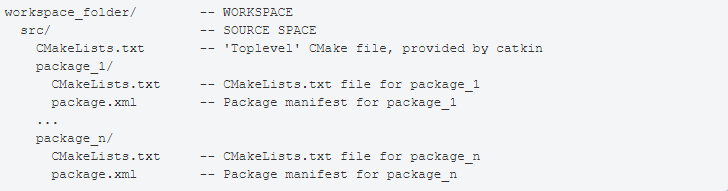
\includegraphics[width=0.8\textwidth]{figs/workspace_example.png}
%    \caption{A work-space in ROS Kinetic is referred to as catkin. This is an example catkin  work-space, showing multiple package %folder structure. The packages can be written in different programming languages(Python, C++, and Lisp, and has experimental %libraries in Java and Lua).}
%    \label{fig:ros-workspace}
%\end{figure}

ROS defines a recommended file structure and software build to promote reuse and ease of sharing in the community. ROS uses the concept of packages (similar to the UNIX operating systems) as the ROS ecosystem's fundamental building block. ROS currently supports the following programming languages Python, C++, and Lisp, and has experimental libraries in Java and Lua.

\subsection{ROS communication}

For the robots to communicate, ROS implements several different communication styles, including synchronous communication over services, asynchronous streaming of data over topics, and storage of data on a Parameter Server. The communication is facilitated by the peer-to-peer network, which can be distributed across machines. The network is based on a graph architecture with a decentralised topology where processing occurs in \textit{nodes} that may publish or subscribe messages, such as multiplex sensor, control, state, planning and actuators. Topics are asynchronous, and \textit{nodes} do not explicitly communicate with each other, services provide synchronous communication, as shown in Figure \ref{fig:ros-basic-concept}.

\begin{figure}[H]
    \centering
    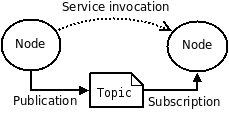
\includegraphics[width=0.4\textwidth]{figs/implementation/ROS_basic_concepts.png}
    \caption{This illustrates the basic node concept.Note that \textit{nodes} do not explicitly communicate with each other, services provide synchronous communication. Taken from \cite{Quigley2009}.}
    \label{fig:ros-basic-concept} 
\end{figure}

The ROS \textit{master} acts as a name-service for the graph; it stores topics and services information for ROS \textit{nodes}, as shown in Figure \ref{fig:ros-basic-concept}. \textit{Nodes} report information to the \textit{master}, and receive messages (include arbitrarily nested structures and arrays) from other \textit{nodes} through the \textit{master}. Nodes need to be registered to the \textit{master} to receive and pass messages. Messages (shown in Figure \ref{fig:ros-master-nodes}) are communicated via topics between \textit{nodes} using publish/subscribe architecture. A node subscribes to a topic, requests a connection through the \textit{master} and connects to a publisher node, hence receiving messages. There may be multiple concurrent \textit{nodes} publishing and subscribing to a single topic, and a node may publish and subscribe to multiple topics. The \textit{master} will also make callbacks to \textit{nodes} when registration information changes, which allows \textit{nodes} to create connections as new \textit{nodes} are registered dynamically. Bag files are used to save and playback ROS messages such as sensor data to develop and test algorithms.


\begin{figure}[H]
    \centering
    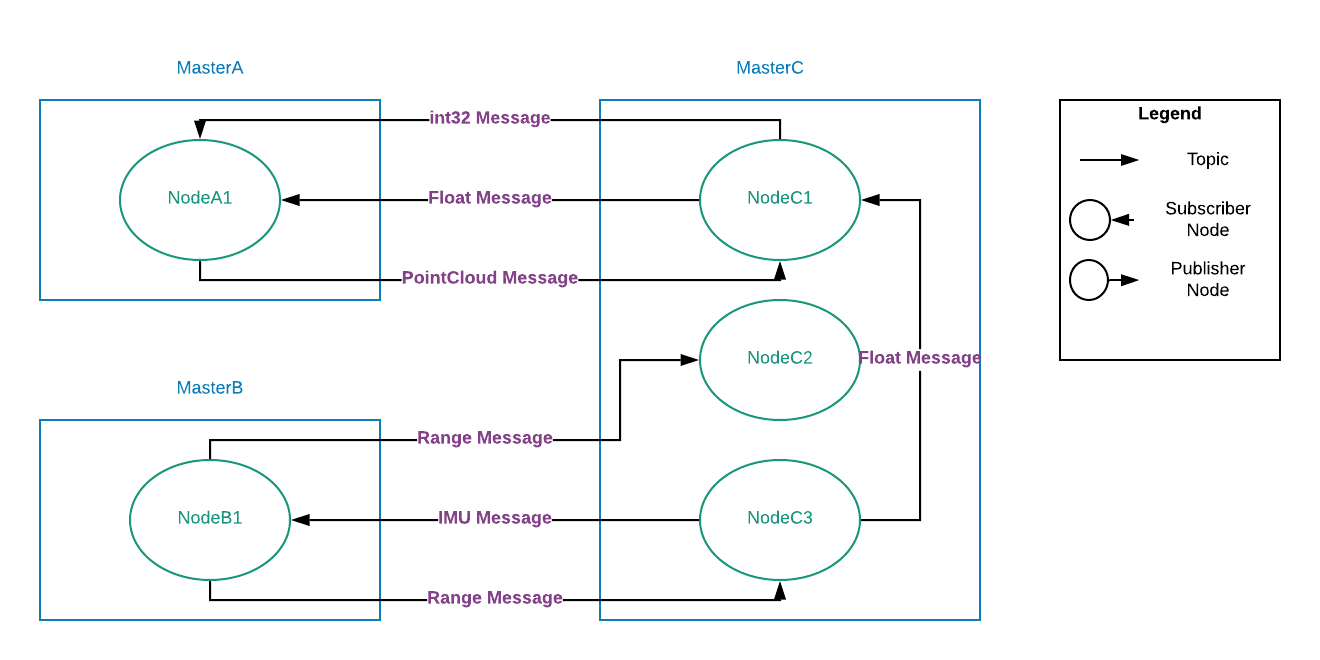
\includegraphics[width=0.9\textwidth]{figs/ros_master_nodes.png}
    \caption{An example of multiple machine/robot ROS implementation architecture. This shows the interaction of nodes between multiple machines/robots. Messages are passed through topics.}
    \label{fig:ros-master-nodes}
\end{figure}

%\begin{figure}[H]
%    \centering
%    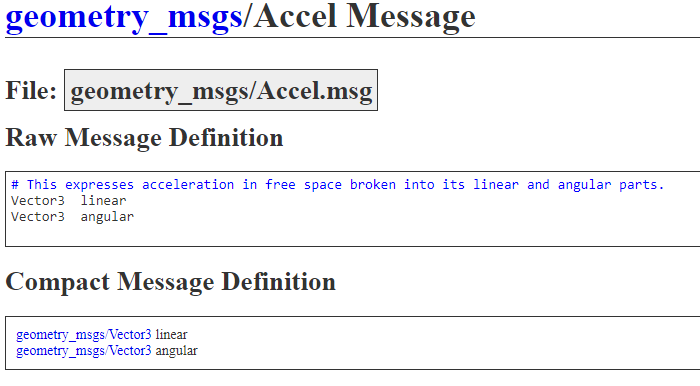
\includegraphics[width=0.7\textwidth]{figs/Ros_message_example.png}
%    \caption{This is an example of an \textit{Accel} message which is as message used to exchange, the linear %and angular vectors are in 3 axes(x, y, z).}
%    \label{fig:ros-message}
%\end{figure}


For example, given that there is a need to control and access data from a Hokuyo laser range-finder, \textit{hokuyo node} driver can be used to talk to the laser and publishes messages of the following type sensor \textit{msgs/LaserScan} to a topic named \textit{scan}. A node (i.e. \textit{laser process} ) can be written to subscribe to messages on the scan topic, to process \textit{msgs/LaserScan} messages. Note that all \textit{hokuyo node} does is to publish messages to the \textit{scan} topic, without knowledge of any nodes subscribed to the topic. On the other hand, the \textit{laser process} node subscribes to \textit{scan} the topic without knowledge of whether any node is publishing. Hence the nodes are decoupled, the nodes can be started, killed and restarted. 

When dealing with multiple robots,  there may be a  need to remap topics for each robot, primarily when robots used the same nodes internally.  ROS supports command-line remapping of names,  which means a compiled program can be reconfigured at run-time to operate in a different graph topology.  For example, the outputs from a laser range-finder for robot1 should not be published to the same topic as the outputs from the laser range-finder of robot2; therefore each robot should publish the scan message to different topics.  Defining a prefix will allow each robot to use a unique name-space for all data and transformations; for example, the two robots' laser scan topic will be robot0/scan, robot1/scan.

\subsection{SLAM in ROS}

Examples of ROS packages dedicated to SLAM algorithms include \(slam\_gmapping\)\footnote{http://wiki.ros.org/gmapping}, \(mrpt\_slam\)\footnote{http://wiki.ros.org/mrpt\_slam?distro=kinetic} and \(hector\_slam\)\footnote{http://wiki.ros.org/hector\_slam}. The stable and commonly used \textit{hector\_slam} is implemented in this work, due to the advantages discussed in Section\ref{sec:hector_slam}. The \textit{hector\_mapping} node is in the package, and it is a SLAM approach that can be implemented without odometry and platforms that exhibit roll/pitch motion(of the sensor, the platform or both) such as quad-rotor UAVs. It leverages the high update rate of modern LIDAR systems like the Hokuyo UTM-30LX and provides 2D pose estimates at the sensors' scan rate. While the algorithm does not provide explicit loop closing ability, it is sufficiently accurate for many real-world scenarios as described in \cite{Eliwa2017}. Furthermore, the system has successfully been used on unmanned ground robots, unmanned surface vehicles, handheld mapping devices and logged data from quad-rotor UAVs and was developed by \cite{Kohlbrecher2011a}.

\subsection{Map and pose exchange}

Robots must be aware of other teammates who join and leave the network, to perform the mapping task cooperatively.  This communication is achieved using a non-distributed \textit{roscore} which is a collection of nodes and programs of a ROS system.  Instead of running \textit{roscore} on each robot a dedicated robot or networked computer will be used to facilitate the communication, to do this \(\$roscore\) is run on the machine chosen to be the master, then the IP of the communication machine is used to run the following \(\$export ROSMASTERURI=http://masterrobotIP:1234/ \)on each robot in the network, to add them to the network.  Even though the master \textit{roscore} has been selected, nodes will still be computed on the individual robots,\textit{roscore} only facilities communication between the teammates.

Assuming that each robot is aware of its ID, i.e. robot1, the robot searches through topics to find which robots exist in the network.   Since robots can leave the network(i.e., map an area with low-quality network link), each robot maintains a list of all the mobile robots.   Assigning a  prefix allows robots to share information such as occupancy grids,  poses, laser scans or messages.  The following information is shared between the robots \textit{OccupancyGrid} and \textit{Pose}.

\subsection{Multi-session}

Multi-session mapping considers the problem of combining the results of mobile robot SLAM missions performed repeatedly over time in the same environment. The goal is to robustly combine multiple maps from different missions in the same environment in a standard coordinate system. Multi-session mapping involves having to deal with the fact that robots over long period missions eventually will be shut down and may revisit areas where they previously mapped. One way of doing multi-session mapping is having a robot localise it is self in a previously-built map. The solution allows the robot to use the same referential, and only one map is created per session; however, this requires the robot the start in the already mapped portion of the environment. In this work, the previously mapped portion of the environment is dealt with as a map from another robot. Hence the robot is not required to start in the portion of the environment previously mapped. Using ROS \(map\_server\), a map is stored and can be retrieved later for use in another process. After a session, the map is stored, and if a map were previously stored on startup, it would be fed into the map merging algorithm.

\subsection{ROS node}

Figure \ref{fig:ros-node-implementation} illustrated the ROS \textit{node} used in this work. The \textit{node} is implemented using Python, the \textit{rospy} library is used to interact with the ROS system. The \textit{node} is designed with parameters to alter the image registration process and parameters to alter the rate at which the \textit{node} runs. In step one the parameters are initialised to default values of which the image registration parameters are determined in Chapter \ref{sec:map-merging}, it is also necessary to know the current robot map topic. The current robot topic is used to ensure that all the partial maps are transformed into that frame. Step two involves getting the list of all the topics which are in the network using \textit{rospy.get\_published\_topics()}; the published topics messages of type \textit{nav\_msgs/OccupancyGrid} are then selected for the map merging process. In step 6 and 7, if there are maps in the network, the maps are then stored using the \textit{map\_server} \textit{node}. In the final step 8, the image registration based map merging algorithm is used. The map merging algorithm is described in Section\ref{sec:map_merging_algorithm}\footnote{GitHub repository: \url{https://github.com/dikokob/DikokoMScEng}}.

\begin{figure}[H]
    \centering
    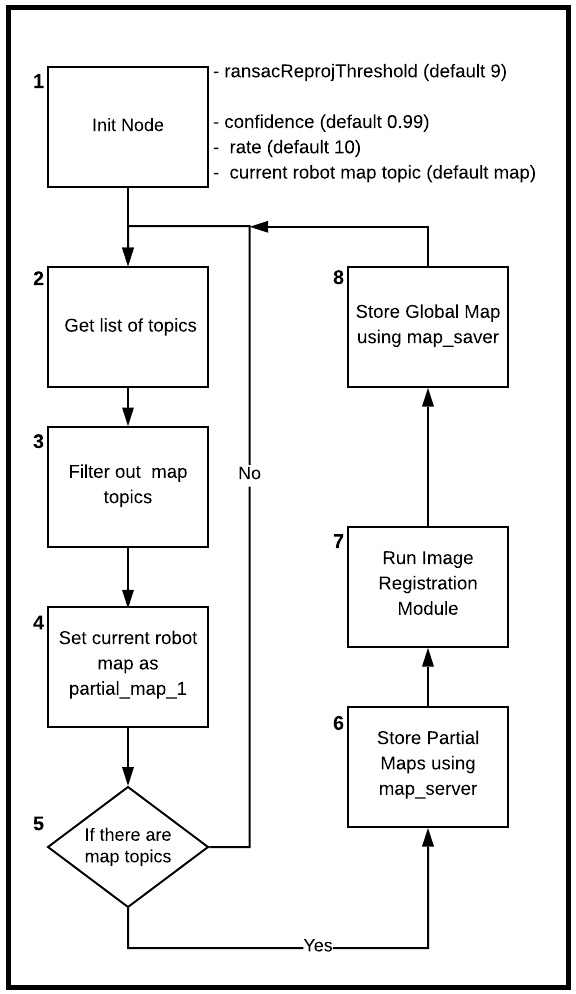
\includegraphics[width=0.6\textwidth]{UCT_MSc_Thesis/figs/implementation/ROSnodeImplementation.jpg}
    \caption{ROS node implementation.}
    \label{fig:ros-node-implementation}
\end{figure}
\


\section{Summary}

In this chapter, a multi-robot multi-session map merging approach is presented. In the next chapter, validation experiments run in simulation and real-world scenarios are discussed. The simulation tests were conducted using two and three partial maps at different resolutions, and so are the real-world experiments.

